\documentclass[
aps,
prl,
reprint,
showpacs,
]{revtex4-1}
\pdfoutput=1

\usepackage{booktabs}
\usepackage{graphicx}
%\usepackage{preprintcover}
\usepackage{multirow}
\usepackage{subfigure}
\usepackage[hyperindex,breaklinks,hidelinks,colorlinks,allcolors=blue]{hyperref} 

%\PreprintCoverPaperTitle{\protect\input{00_Title.tex}}
%
%\PreprintIdNumber{CERN-PH-EP-2014-047}
%
%\PreprintJournalName{Phys. Rev. Lett.}
%
%\PreprintCoverAbstract{\input{00_Abstract}}

\begin{document}

\title{Search for Pair Production of Third-Generation Scalar Leptoquarks Decaying to $b \tau b \tau $ with the ATLAS Detector}

\author{Garrett W. Merz}
\collaboration{ATLAS Collaboration}

\begin{abstract}
\noindent Recent observations at Brookhaven's E821 experiment and CERN's LHCb experiment have reinvigorated theoretical interest in leptoquarks, hypothetical particles that couple the lepton and quark sectors. We discuss an ongoing search for leptoquark pair production at ATLAS and its implications.
\end{abstract}

%\pacs{13.38.Dg}

\maketitle

In June of 2017, the LHCb collaboration reported that they had observed a $2.1\sigma$ deviation from the Standard Model prediction in their measurement of R(D*), the ratio of the $B^0\rightarrow D^*^- \tau^+ \nu_\tau$ branching fraction to the $B^0\rightarrow D^*^- \mu^+ \nu_\mu$ branching fraction \cite{LHCbRD*}. According to the principle of lepton universality, aside from a phase space factor originating from the different masses of the charged leptons, these two decays should occur with equal frequency; however, observed results indicated that this may not in fact be the case. The deviation observed suggests a potential violation of lepton universality, joining past measurements from the BaBar and Belle collaborations in casting doubt on the accuracy of this Standard Model prediction \cite{BaBar, Belle}.


\begin{figure}[h]
\includegraphics[width=.95\linewidth]{lhcbplot} 
\caption{Measurements of R(D*) as they compare to the Standard Model prediction \cite{LHCbRD*}.}
\label{fig:landscape}
\end{figure}


One proposed explanation for these deviations is the introduction of leptoquarks, particles which carry both lepton number and baryon number. By providing another avenue for quarks to decay into leptons, these particles can modify the value of R(D*) to better conform with observed results \cite{Ciezarek}.
\begin{figure}[h]
\includegraphics[width=.95\linewidth]{RDSMLQ} 
\caption{The decay of a B meson to a charged lepton, a neutrino, and a D meson, via Standard Model mechanisms (top) and via radiation of a leptoquark (bottom) \cite{Ciezarek}.}
\label{fig:landscape}
\end{figure}


Further motivation for leptoquark searches comes from another noteworthy experimental discrepancy in high-energy physics: In 2004, the E281 experiment at Brookhaven National Laboratory observed a $3.5\sigma$ deviation from the Standard Model prediction in their measurement of the muon anomalous magnetic moment. This quantity, the effect of quantum loop corrections on the muon's magnetic dipole moment, would be highly sensitive to the existence of beyond-the-Standard-Model particles. Additional loop corrections involving leptoquarks may be able to explain some or all of this discrepancy, and, as such, provide further motivation for a direct leptoquark search \cite{Cheung}.


Many Standard Model extensions feature leptoquarks, including the Pati-Salam model and SU(5) and SO(10) Grand Unified Theories \cite{Sakaki}. Some of the simplest leptoquark models predict the existence of one or more scalar leptoquarks, which carry spin zero and couple to different generations of fermions. 


A recent $hh \rightarrow b\tau b\tau$ search conducted with the ATLAS detector offers an analysis framework that is easily adaptable to a search for third-generation leptoquark pair production \cite{hh}. The last ATLAS search for third generation leptoquarks decaying to $b\tau b\tau$ excluded leptoquarks below a mass of 534 GeV using approximately $5fb^{-1}$ of 7 TeV data \cite{lastATLAS}, while the last CMS search for third generation leptoquarks decaying to $b\tau b\tau$ excluded leptoquarks below a mass of 740 GeV using approximately $5fb^{-1}$ of 7 TeV data \cite{lastATLAS}. This search, which will be the first such search conducted during the Run II of the LHC, will be conducted with 36.1 $fb^-1$ of 13 TeV data, and, as such, is expected to provide much stronger limits than previous searches.


\begin{figure}[h]
\includegraphics[width=.95\linewidth]{LQ3ggF} 
\caption{The dominant pair-production mode for $LQ3 \rightarrow b \tau b \tau$}
\label{fig:landscape}
\end{figure}


As in the $hh$ analysis, the search is broken up into two channels, one in which both taus decay hadronically, dubbed $had-had$, and one in which one tau decays leptonically, dubbed $lep-had$. Due to its comparatively small branching ratio, we do not consider a $lep-lep$ channel, in which both taus decay leptonically.

In the lep-had channel, we utilize the Single Lepton Trigger (SLT), which stores events possessing one of the following qualities:

\begin{itemize}
    \item in early (late) periods, an electron with pT $>$ 24 (26) GeV that falls into the ‘medium’ ('tight') electron ID category, and the ‘loose’ isolation category, both of which are defined in \cite{elIDs}
    \item an electron with pT $>$ 120 (140) GeV and ‘medium’ ID, no isolation requirements
    \item an electron with pT $>$ 60 and ‘medium’ ID, no isolation requirements
    \item a muon with pT $>$ 24 (26) GeV and 'loose' isolation
\end{itemize}

In addition to these basic trigger requirements, we require 



Due to the relatively small expected signal contribution, a Boosted Decision Tree (BDT) is used to distinguish signal from background. We train the BDT 

















\begin{figure}[h]
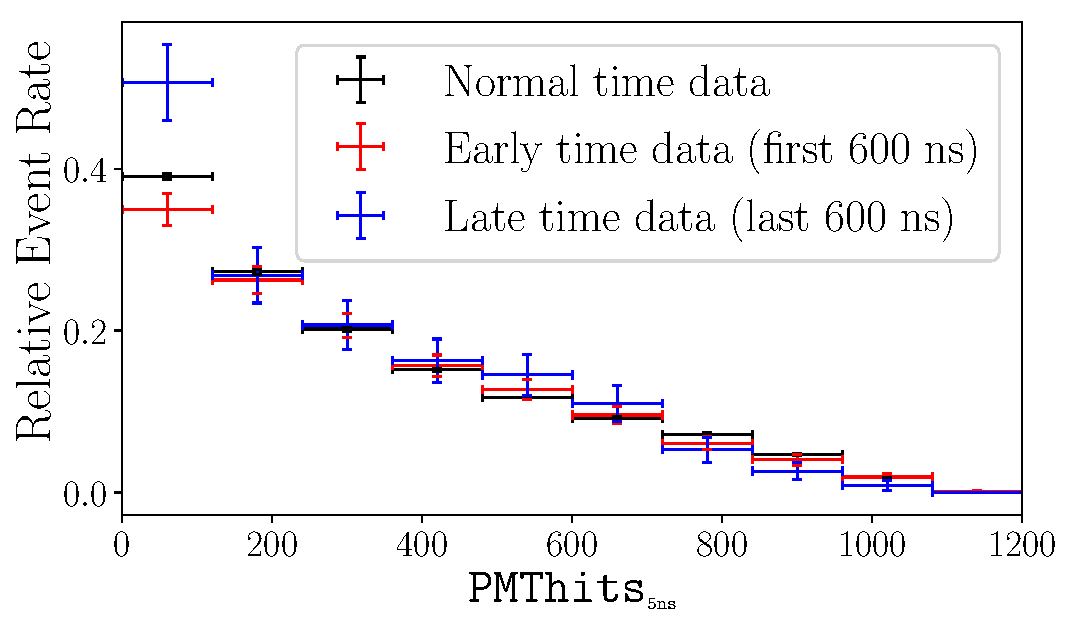
\includegraphics[width=.95\linewidth]{img/observation} 
\caption{CAPTION}
\label{fig:obs}
\end{figure}


 Table \ref{tab:exp}.

\begin{table*}
  \label{tab:exp}
  \begin{ruledtabular}
  \newcommand{\twrw}[1]{\multirow{2}{*}{#1}}
  \begin{tabular}{lccc}
  Experiment & Exposure (POT) & Distance from source (m) & 236 MeV $\nu_\mu$ events \\
    \hline
MiniBooNE & $2.62\times 10^{20}$ (1 year) & 86 m& $3500\pm1500$ \\
MicroBooNE & $1.2\times 10^{21}$ (2 years) & 102 m & 2300 \\
JSNS$^2$ & $1.125\times 10^{23}$ (3 years) & 24 m  & 30-60k \\

  \end{tabular}
  \end{ruledtabular}
    \caption{A summary of experiments that can detect KDAR neutrinos and the event rates expected.}
\end{table*}

\begin{thebibliography}{9}

\bibitem{LHCbRD*}
R. Aaij et. al. [LHCb Collaboration]. LHCb-PAPER-2017-017.

\bibitem{BaBar}
R. Aaij et. al. [LHCb Collaboration]. LHCb-PAPER-2017-017.

\bibitem{Belle}
R. Aaij et. al. [LHCb Collaboration]. LHCb-PAPER-2017-017.

\bibitem{Ciezarek}
G. Ciezarek et. al. A challenge to lepton universality in B-meson decays. Nature 546, 227–233.

\bibitem{Sakaki}
Y. Sakaki et. al. Testing leptoquark models in B0 → D*-τ+ντ . Phys. Rev. D 88, 094012

\bibitem{Cheung}
K.-M. Cheung, Muon Anomalous Magnetic Moment and Leptoquark Solutions. Phys. Rev. D 64, 033001

\bibitem{elIDs}
CERN-EP-2016-262















\end{thebibliography}

\end{document}
